% Created by tikzDevice version 0.12.6 on 2026-05-14 20:37:55
% !TEX encoding = UTF-8 Unicode
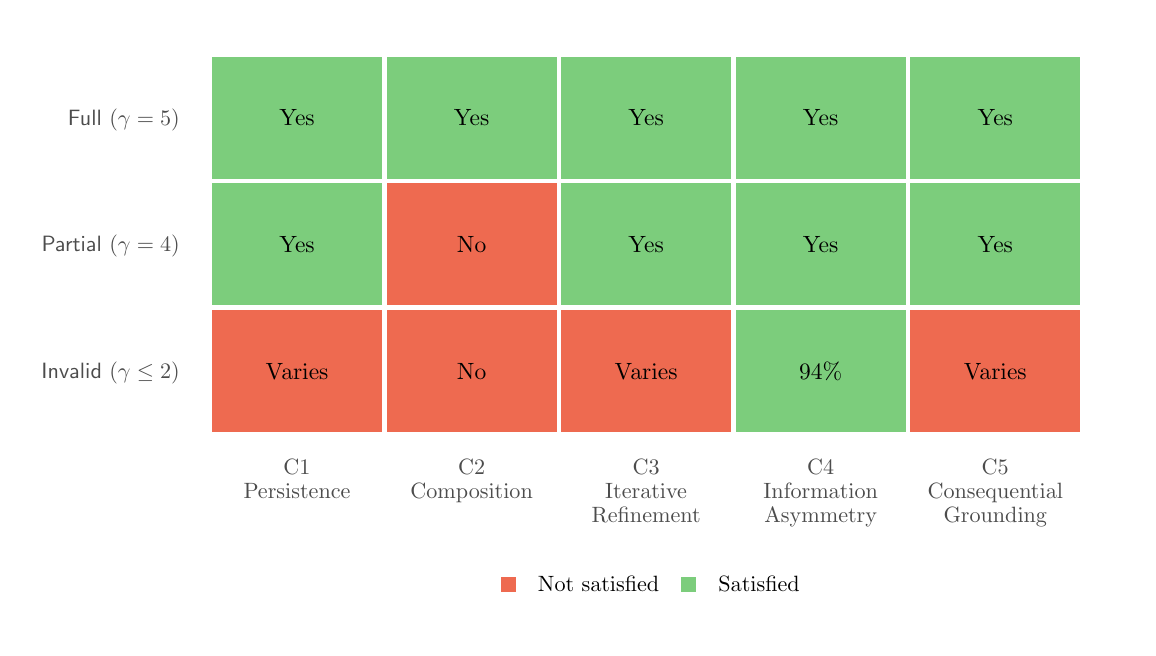
\begin{tikzpicture}[x=1pt,y=1pt]
\definecolor{fillColor}{RGB}{255,255,255}
\path[use as bounding box,fill=fillColor,fill opacity=0.00] (0,0) rectangle (397.48,216.81);
\begin{scope}
\path[clip] (  0.00,  0.00) rectangle (397.48,216.81);
\definecolor{fillColor}{RGB}{255,255,255}

\path[fill=fillColor] ( -0.00,  0.00) rectangle (397.48,216.81);
\end{scope}
\begin{scope}
\path[clip] ( 59.48, 65.23) rectangle (387.48,211.81);
\definecolor{drawColor}{RGB}{255,255,255}
\definecolor{fillColor}{RGB}{124,205,124}

\path[draw=drawColor,line width= 1.7pt,fill=fillColor] ( 65.79,161.42) rectangle (128.87,207.23);

\path[draw=drawColor,line width= 1.7pt,fill=fillColor] (128.87,161.42) rectangle (191.95,207.23);

\path[draw=drawColor,line width= 1.7pt,fill=fillColor] (191.95,161.42) rectangle (255.02,207.23);

\path[draw=drawColor,line width= 1.7pt,fill=fillColor] (255.02,161.42) rectangle (318.10,207.23);

\path[draw=drawColor,line width= 1.7pt,fill=fillColor] (318.10,161.42) rectangle (381.18,207.23);

\path[draw=drawColor,line width= 1.7pt,fill=fillColor] ( 65.79,115.61) rectangle (128.87,161.42);
\definecolor{fillColor}{RGB}{238,106,80}

\path[draw=drawColor,line width= 1.7pt,fill=fillColor] (128.87,115.61) rectangle (191.95,161.42);
\definecolor{fillColor}{RGB}{124,205,124}

\path[draw=drawColor,line width= 1.7pt,fill=fillColor] (191.95,115.61) rectangle (255.02,161.42);

\path[draw=drawColor,line width= 1.7pt,fill=fillColor] (255.02,115.61) rectangle (318.10,161.42);

\path[draw=drawColor,line width= 1.7pt,fill=fillColor] (318.10,115.61) rectangle (381.18,161.42);
\definecolor{fillColor}{RGB}{238,106,80}

\path[draw=drawColor,line width= 1.7pt,fill=fillColor] ( 65.79, 69.81) rectangle (128.87,115.61);

\path[draw=drawColor,line width= 1.7pt,fill=fillColor] (128.87, 69.81) rectangle (191.95,115.61);

\path[draw=drawColor,line width= 1.7pt,fill=fillColor] (191.95, 69.81) rectangle (255.02,115.61);
\definecolor{fillColor}{RGB}{124,205,124}

\path[draw=drawColor,line width= 1.7pt,fill=fillColor] (255.02, 69.81) rectangle (318.10,115.61);
\definecolor{fillColor}{RGB}{238,106,80}

\path[draw=drawColor,line width= 1.7pt,fill=fillColor] (318.10, 69.81) rectangle (381.18,115.61);
\definecolor{drawColor}{RGB}{0,0,0}

\node[text=drawColor,anchor=base,inner sep=0pt, outer sep=0pt, scale=  0.85] at ( 97.33,181.39) {Yes};

\node[text=drawColor,anchor=base,inner sep=0pt, outer sep=0pt, scale=  0.85] at (160.41,181.39) {Yes};

\node[text=drawColor,anchor=base,inner sep=0pt, outer sep=0pt, scale=  0.85] at (223.48,181.39) {Yes};

\node[text=drawColor,anchor=base,inner sep=0pt, outer sep=0pt, scale=  0.85] at (286.56,181.39) {Yes};

\node[text=drawColor,anchor=base,inner sep=0pt, outer sep=0pt, scale=  0.85] at (349.64,181.39) {Yes};

\node[text=drawColor,anchor=base,inner sep=0pt, outer sep=0pt, scale=  0.85] at ( 97.33,135.58) {Yes};

\node[text=drawColor,anchor=base,inner sep=0pt, outer sep=0pt, scale=  0.85] at (160.41,135.58) {No};

\node[text=drawColor,anchor=base,inner sep=0pt, outer sep=0pt, scale=  0.85] at (223.48,135.58) {Yes};

\node[text=drawColor,anchor=base,inner sep=0pt, outer sep=0pt, scale=  0.85] at (286.56,135.58) {Yes};

\node[text=drawColor,anchor=base,inner sep=0pt, outer sep=0pt, scale=  0.85] at (349.64,135.58) {Yes};

\node[text=drawColor,anchor=base,inner sep=0pt, outer sep=0pt, scale=  0.85] at ( 97.33, 89.77) {Varies};

\node[text=drawColor,anchor=base,inner sep=0pt, outer sep=0pt, scale=  0.85] at (160.41, 89.77) {No};

\node[text=drawColor,anchor=base,inner sep=0pt, outer sep=0pt, scale=  0.85] at (223.48, 89.77) {Varies};

\node[text=drawColor,anchor=base,inner sep=0pt, outer sep=0pt, scale=  0.85] at (286.56, 89.77) {94\%};

\node[text=drawColor,anchor=base,inner sep=0pt, outer sep=0pt, scale=  0.85] at (349.64, 89.77) {Varies};
\end{scope}
\begin{scope}
\path[clip] (  0.00,  0.00) rectangle (397.48,216.81);
\definecolor{drawColor}{gray}{0.30}

\node[text=drawColor,anchor=base east,inner sep=0pt, outer sep=0pt, scale=  0.80] at ( 54.98, 89.96) {$\mathsf{Invalid}$ ($\gamma \leq 2$)};

\node[text=drawColor,anchor=base east,inner sep=0pt, outer sep=0pt, scale=  0.80] at ( 54.98,135.76) {$\mathsf{Partial}$ ($\gamma=4$)};

\node[text=drawColor,anchor=base east,inner sep=0pt, outer sep=0pt, scale=  0.80] at ( 54.98,181.57) {$\mathsf{Full}$ ($\gamma=5$)};
\end{scope}
\begin{scope}
\path[clip] (  0.00,  0.00) rectangle (397.48,216.81);
\definecolor{drawColor}{gray}{0.30}

\node[text=drawColor,anchor=base,inner sep=0pt, outer sep=0pt, scale=  0.80] at ( 97.33, 55.22) {C1};

\node[text=drawColor,anchor=base,inner sep=0pt, outer sep=0pt, scale=  0.80] at ( 97.33, 46.58) {Persistence};

\node[text=drawColor,anchor=base,inner sep=0pt, outer sep=0pt, scale=  0.80] at (160.41, 55.22) {C2};

\node[text=drawColor,anchor=base,inner sep=0pt, outer sep=0pt, scale=  0.80] at (160.41, 46.58) {Composition};

\node[text=drawColor,anchor=base,inner sep=0pt, outer sep=0pt, scale=  0.80] at (223.48, 55.22) {C3};

\node[text=drawColor,anchor=base,inner sep=0pt, outer sep=0pt, scale=  0.80] at (223.48, 46.58) {Iterative};

\node[text=drawColor,anchor=base,inner sep=0pt, outer sep=0pt, scale=  0.80] at (223.48, 37.94) {Refinement};

\node[text=drawColor,anchor=base,inner sep=0pt, outer sep=0pt, scale=  0.80] at (286.56, 55.22) {C4};

\node[text=drawColor,anchor=base,inner sep=0pt, outer sep=0pt, scale=  0.80] at (286.56, 46.58) {Information};

\node[text=drawColor,anchor=base,inner sep=0pt, outer sep=0pt, scale=  0.80] at (286.56, 37.94) {Asymmetry};

\node[text=drawColor,anchor=base,inner sep=0pt, outer sep=0pt, scale=  0.80] at (349.64, 55.22) {C5};

\node[text=drawColor,anchor=base,inner sep=0pt, outer sep=0pt, scale=  0.80] at (349.64, 46.58) {Consequential};

\node[text=drawColor,anchor=base,inner sep=0pt, outer sep=0pt, scale=  0.80] at (349.64, 37.94) {Grounding};
\end{scope}
\begin{scope}
\path[clip] (  0.00,  0.00) rectangle (397.48,216.81);
\definecolor{drawColor}{RGB}{255,255,255}
\definecolor{fillColor}{RGB}{238,106,80}

\path[draw=drawColor,line width= 1.7pt,fill=fillColor] (170.12, 12.13) rectangle (177.24, 19.25);
\end{scope}
\begin{scope}
\path[clip] (  0.00,  0.00) rectangle (397.48,216.81);
\definecolor{drawColor}{RGB}{255,255,255}
\definecolor{fillColor}{RGB}{124,205,124}

\path[draw=drawColor,line width= 1.7pt,fill=fillColor] (235.36, 12.13) rectangle (242.47, 19.25);
\end{scope}
\begin{scope}
\path[clip] (  0.00,  0.00) rectangle (397.48,216.81);
\definecolor{drawColor}{RGB}{0,0,0}

\node[text=drawColor,anchor=base west,inner sep=0pt, outer sep=0pt, scale=  0.80] at (184.37, 12.94) {Not satisfied};
\end{scope}
\begin{scope}
\path[clip] (  0.00,  0.00) rectangle (397.48,216.81);
\definecolor{drawColor}{RGB}{0,0,0}

\node[text=drawColor,anchor=base west,inner sep=0pt, outer sep=0pt, scale=  0.80] at (249.61, 12.94) {Satisfied};
\end{scope}
\end{tikzpicture}
